\documentclass{standalone}
\usepackage{tikz}
\usetikzlibrary{patterns, positioning}

\begin{document}
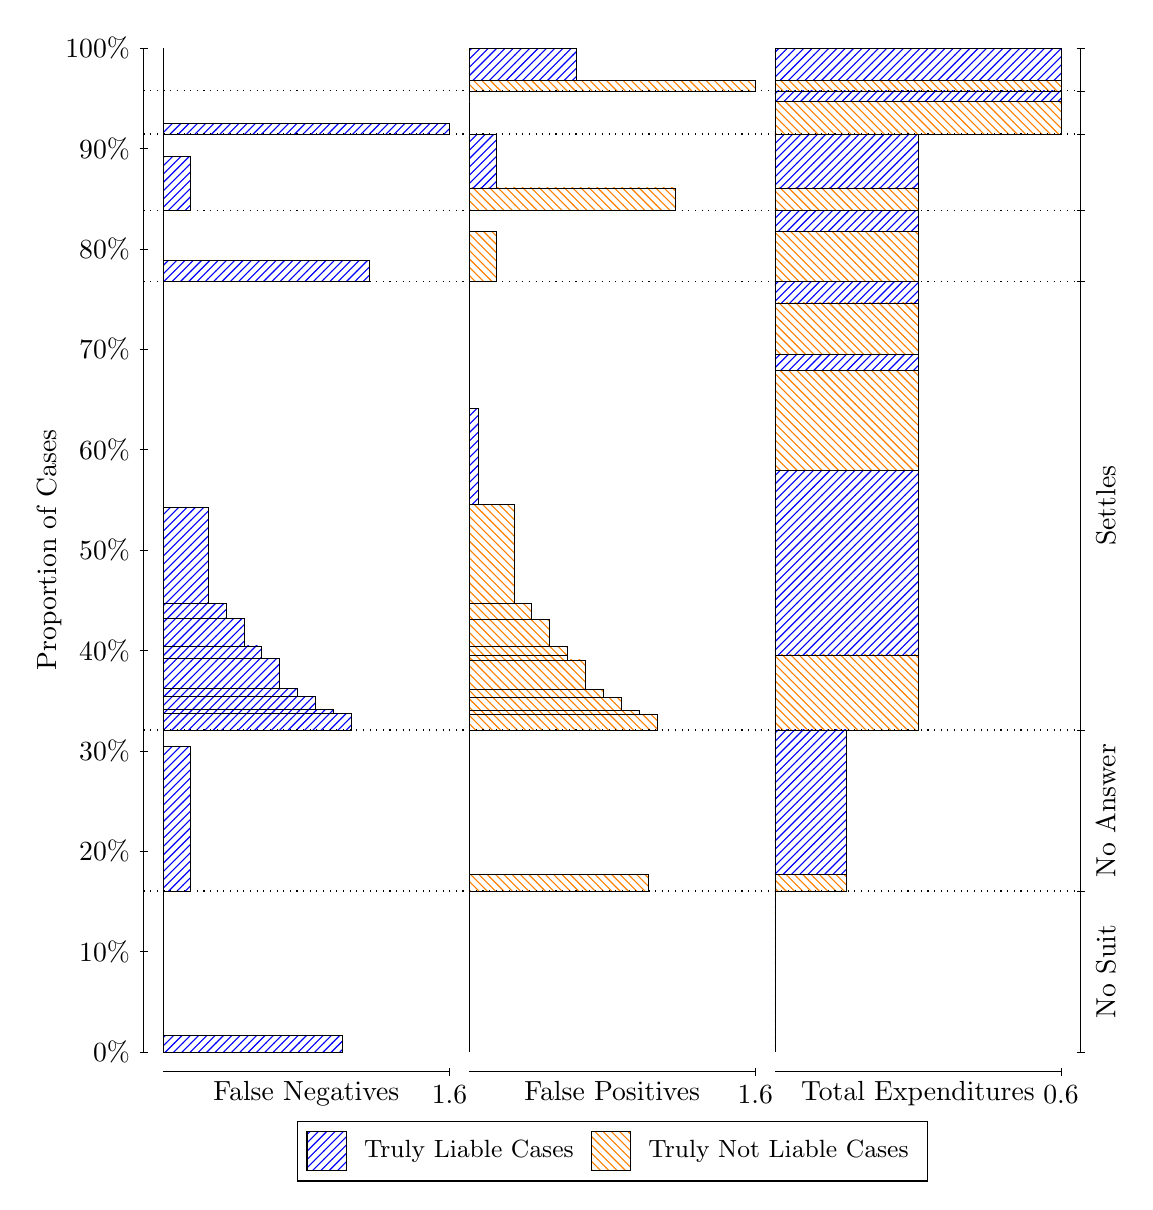
\begin{tikzpicture}
\draw[black, very thin] (1.5,1.75) -- (1.5,14.5);
\node[rotate=90, anchor=center] at (0.3, 8.125) {Proportion of Cases};
\draw[black, very thin] (1.45,1.75) -- (1.55,1.75);
\node[anchor=east] at (1.45, 1.75) {0\%};
\draw[black, very thin] (1.45,3.025) -- (1.55,3.025);
\node[anchor=east] at (1.45, 3.025) {10\%};
\draw[black, very thin] (1.45,4.3) -- (1.55,4.3);
\node[anchor=east] at (1.45, 4.3) {20\%};
\draw[black, very thin] (1.45,5.575) -- (1.55,5.575);
\node[anchor=east] at (1.45, 5.575) {30\%};
\draw[black, very thin] (1.45,6.85) -- (1.55,6.85);
\node[anchor=east] at (1.45, 6.85) {40\%};
\draw[black, very thin] (1.45,8.125) -- (1.55,8.125);
\node[anchor=east] at (1.45, 8.125) {50\%};
\draw[black, very thin] (1.45,9.4) -- (1.55,9.4);
\node[anchor=east] at (1.45, 9.4) {60\%};
\draw[black, very thin] (1.45,10.675) -- (1.55,10.675);
\node[anchor=east] at (1.45, 10.675) {70\%};
\draw[black, very thin] (1.45,11.95) -- (1.55,11.95);
\node[anchor=east] at (1.45, 11.95) {80\%};
\draw[black, very thin] (1.45,13.225) -- (1.55,13.225);
\node[anchor=east] at (1.45, 13.225) {90\%};
\draw[black, very thin] (1.45,14.5) -- (1.55,14.5);
\node[anchor=east] at (1.45, 14.5) {100\%};

\draw[black, very thin] (13.4,1.75) -- (13.4,14.5);
\draw[black, very thin] (13.35,1.75) -- (13.45,1.75);
\node[anchor=west] at (13.35, 1.75) {};
\draw[black, very thin] (13.35,3.7939) -- (13.45,3.7939);
\node[anchor=west] at (13.35, 3.7939) {};
\draw[black, very thin] (13.35,5.8391) -- (13.45,5.8391);
\node[anchor=west] at (13.35, 5.8391) {};
\draw[black, very thin] (13.35,11.538) -- (13.45,11.538);
\node[anchor=west] at (13.35, 11.538) {};
\draw[black, very thin] (13.35,12.436) -- (13.45,12.436);
\node[anchor=west] at (13.35, 12.436) {};
\draw[black, very thin] (13.35,13.408) -- (13.45,13.408);
\node[anchor=west] at (13.35, 13.408) {};
\draw[black, very thin] (13.35,13.955) -- (13.45,13.955);
\node[anchor=west] at (13.35, 13.955) {};
\draw[black, very thin] (13.35,14.5) -- (13.45,14.5);
\node[anchor=west] at (13.35, 14.5) {};

\draw[black, very thin, pattern color=blue, pattern=north east lines] (1.75,1.75) rectangle (4.0208,1.965);
\draw[black, very thin, pattern color=orange, pattern=north west lines] (1.75,1.965) rectangle (1.75,3.7939);
\draw[black, very thin, pattern color=blue, pattern=north east lines] (1.75,3.7939) rectangle (2.0906,5.629);
\draw[black, very thin, pattern color=orange, pattern=north west lines] (1.75,5.629) rectangle (1.75,5.8391);
\draw[black, very thin, pattern color=blue, pattern=north east lines] (1.75,5.8391) rectangle (4.1344,6.0484);
\draw[black, very thin, pattern color=blue, pattern=north east lines] (1.75,6.0484) rectangle (3.9073,6.0995);
\draw[black, very thin, pattern color=blue, pattern=north east lines] (1.75,6.0995) rectangle (3.6802,6.2627);
\draw[black, very thin, pattern color=blue, pattern=north east lines] (1.75,6.2627) rectangle (3.4531,6.3693);
\draw[black, very thin, pattern color=blue, pattern=north east lines] (1.75,6.3693) rectangle (3.226,6.7499);
\draw[black, very thin, pattern color=blue, pattern=north east lines] (1.75,6.7499) rectangle (2.999,6.9082);
\draw[black, very thin, pattern color=blue, pattern=north east lines] (1.75,6.9082) rectangle (2.7719,7.2536);
\draw[black, very thin, pattern color=blue, pattern=north east lines] (1.75,7.2536) rectangle (2.5448,7.4517);
\draw[black, very thin, pattern color=blue, pattern=north east lines] (1.75,7.4517) rectangle (2.3177,8.6688);
\draw[black, very thin, pattern color=orange, pattern=north west lines] (1.75,8.6688) rectangle (1.75,11.538);
\draw[black, very thin, pattern color=blue, pattern=north east lines] (1.75,11.538) rectangle (4.3615,11.806);
\draw[black, very thin, pattern color=orange, pattern=north west lines] (1.75,11.806) rectangle (1.75,12.436);
\draw[black, very thin, pattern color=blue, pattern=north east lines] (1.75,12.436) rectangle (2.0906,13.119);
\draw[black, very thin, pattern color=orange, pattern=north west lines] (1.75,13.119) rectangle (1.75,13.408);
\draw[black, very thin, pattern color=blue, pattern=north east lines] (1.75,13.408) rectangle (5.3833,13.545);
\draw[black, very thin, pattern color=orange, pattern=north west lines] (1.75,13.545) rectangle (1.75,13.955);
\draw[black, very thin, pattern color=orange, pattern=north west lines] (1.75,13.955) rectangle (1.75,14.092);
\draw[black, very thin, pattern color=blue, pattern=north east lines] (1.75,14.092) rectangle (1.75,14.5);
\draw[black, very thin, pattern color=orange, pattern=north west lines] (5.6333,1.75) rectangle (5.6333,3.5789);
\draw[black, very thin, pattern color=blue, pattern=north east lines] (5.6333,3.5789) rectangle (5.6333,3.7939);
\draw[black, very thin, pattern color=orange, pattern=north west lines] (5.6333,3.7939) rectangle (7.9042,4.004);
\draw[black, very thin, pattern color=blue, pattern=north east lines] (5.6333,4.004) rectangle (5.6333,5.8391);
\draw[black, very thin, pattern color=orange, pattern=north west lines] (5.6333,5.8391) rectangle (8.0177,6.0416);
\draw[black, very thin, pattern color=orange, pattern=north west lines] (5.6333,6.0416) rectangle (7.7906,6.0911);
\draw[black, very thin, pattern color=orange, pattern=north west lines] (5.6333,6.0911) rectangle (7.5635,6.2496);
\draw[black, very thin, pattern color=orange, pattern=north west lines] (5.6333,6.2496) rectangle (7.3365,6.3543);
\draw[black, very thin, pattern color=orange, pattern=north west lines] (5.6333,6.3543) rectangle (7.1094,6.729);
\draw[black, very thin, pattern color=orange, pattern=north west lines] (5.6333,6.729) rectangle (6.8823,6.7941);
\draw[black, very thin, pattern color=orange, pattern=north west lines] (5.6333,6.7941) rectangle (6.8823,6.8991);
\draw[black, very thin, pattern color=orange, pattern=north west lines] (5.6333,6.8991) rectangle (6.6552,7.2457);
\draw[black, very thin, pattern color=orange, pattern=north west lines] (5.6333,7.2457) rectangle (6.4281,7.4443);
\draw[black, very thin, pattern color=orange, pattern=north west lines] (5.6333,7.4443) rectangle (6.201,8.7085);
\draw[black, very thin, pattern color=blue, pattern=north east lines] (5.6333,8.7085) rectangle (5.7469,9.9256);
\draw[black, very thin, pattern color=blue, pattern=north east lines] (5.6333,9.9256) rectangle (5.6333,11.538);
\draw[black, very thin, pattern color=orange, pattern=north west lines] (5.6333,11.538) rectangle (5.974,12.169);
\draw[black, very thin, pattern color=blue, pattern=north east lines] (5.6333,12.169) rectangle (5.6333,12.436);
\draw[black, very thin, pattern color=orange, pattern=north west lines] (5.6333,12.436) rectangle (8.2448,12.725);
\draw[black, very thin, pattern color=blue, pattern=north east lines] (5.6333,12.725) rectangle (5.974,13.408);
\draw[black, very thin, pattern color=orange, pattern=north west lines] (5.6333,13.408) rectangle (5.6333,13.819);
\draw[black, very thin, pattern color=blue, pattern=north east lines] (5.6333,13.819) rectangle (5.6333,13.955);
\draw[black, very thin, pattern color=orange, pattern=north west lines] (5.6333,13.955) rectangle (9.2667,14.092);
\draw[black, very thin, pattern color=blue, pattern=north east lines] (5.6333,14.092) rectangle (6.9958,14.5);
\draw[black, very thin, pattern color=orange, pattern=north west lines] (9.5167,1.75) rectangle (9.5167,3.5789);
\draw[black, very thin, pattern color=blue, pattern=north east lines] (9.5167,3.5789) rectangle (9.5167,3.7939);
\draw[black, very thin, pattern color=orange, pattern=north west lines] (9.5167,3.7939) rectangle (10.425,4.004);
\draw[black, very thin, pattern color=blue, pattern=north east lines] (9.5167,4.004) rectangle (10.425,5.8391);
\draw[black, very thin, pattern color=orange, pattern=north west lines] (9.5167,5.8391) rectangle (11.333,6.7941);
\draw[black, very thin, pattern color=blue, pattern=north east lines] (9.5167,6.7941) rectangle (11.333,9.1389);
\draw[black, very thin, pattern color=orange, pattern=north west lines] (9.5167,9.1389) rectangle (11.333,10.403);
\draw[black, very thin, pattern color=blue, pattern=north east lines] (9.5167,10.403) rectangle (11.333,10.612);
\draw[black, very thin, pattern color=orange, pattern=north west lines] (9.5167,10.612) rectangle (11.333,11.263);
\draw[black, very thin, pattern color=blue, pattern=north east lines] (9.5167,11.263) rectangle (11.333,11.538);
\draw[black, very thin, pattern color=orange, pattern=north west lines] (9.5167,11.538) rectangle (11.333,12.169);
\draw[black, very thin, pattern color=blue, pattern=north east lines] (9.5167,12.169) rectangle (11.333,12.436);
\draw[black, very thin, pattern color=orange, pattern=north west lines] (9.5167,12.436) rectangle (11.333,12.725);
\draw[black, very thin, pattern color=blue, pattern=north east lines] (9.5167,12.725) rectangle (11.333,13.408);
\draw[black, very thin, pattern color=orange, pattern=north west lines] (9.5167,13.408) rectangle (13.15,13.819);
\draw[black, very thin, pattern color=blue, pattern=north east lines] (9.5167,13.819) rectangle (13.15,13.955);
\draw[black, very thin, pattern color=orange, pattern=north west lines] (9.5167,13.955) rectangle (13.15,14.092);
\draw[black, very thin, pattern color=blue, pattern=north east lines] (9.5167,14.092) rectangle (13.15,14.5);
\draw[black, dotted] (1.5,3.7939) -- (13.4,3.7939);
\draw[black, dotted] (1.5,5.8391) -- (13.4,5.8391);
\draw[black, dotted] (1.5,11.538) -- (13.4,11.538);
\draw[black, dotted] (1.5,12.436) -- (13.4,12.436);
\draw[black, dotted] (1.5,13.408) -- (13.4,13.408);
\draw[black, dotted] (1.5,13.955) -- (13.4,13.955);
\draw[black, very thin] (1.75,1.5) -- (5.3833,1.5);
\node[anchor=north] at (3.5667, 1.5) {False Negatives};
\draw[black, very thin] (5.3833,1.45) -- (5.3833,1.55);
\node[anchor=north] at (5.3833, 1.45) {1.6};

\draw[black, very thin] (5.6333,1.5) -- (9.2667,1.5);
\node[anchor=north] at (7.45, 1.5) {False Positives};
\draw[black, very thin] (9.2667,1.45) -- (9.2667,1.55);
\node[anchor=north] at (9.2667, 1.45) {1.6};

\draw[black, very thin] (9.5167,1.5) -- (13.15,1.5);
\node[anchor=north] at (11.333, 1.5) {Total Expenditures};
\draw[black, very thin] (13.15,1.45) -- (13.15,1.55);
\node[anchor=north] at (13.15, 1.45) {0.6};

\node[black, centered, rotate=90] at (13.72, 2.772) {No Suit};
\node[black, centered, rotate=90] at (13.72, 4.8165) {No Answer};
\node[black, centered, rotate=90] at (13.72, 8.6886) {Settles};





\draw (7.449999999999999,1.5) node[draw=none] (baseCoordinate) {};
\begin{scope}[align=center]
        \matrix[scale=0.5, draw=black, below=0.5cm of baseCoordinate, nodes={draw}, column sep=0.1cm]{
            \node[rectangle, draw, minimum width=0.5cm, minimum height=0.5cm, pattern=north east lines, pattern color=blue] {}; &
            \node[draw=none, font=\small] (B) {Truly Liable Cases}; &
            \node[rectangle, draw, minimum width=0.5cm, minimum height=0.5cm, pattern=north west lines, pattern color=orange] {}; &
            \node[draw=none, font=\small] (B) {Truly Not Liable Cases}; \\
            };
\end{scope}

\end{tikzpicture}
\end{document}